\documentclass[]{article} 
\usepackage{pgfplots} 
\usepgfplotslibrary{external} 
\tikzexternalize 
\usepgfplotslibrary{fillbetween}
\usepackage{tikz} 
\usepackage{amsmath} 
\usepackage{pgfplots} 
\usetikzlibrary{calc} 
\pgfplotsset{compat = newest,every x tick label/.append style={font=\scriptsize,color = white},every y tick label/.append style={font=\scriptsize}, every axis plot post/.style={line join=round}}
\begin{document} 
	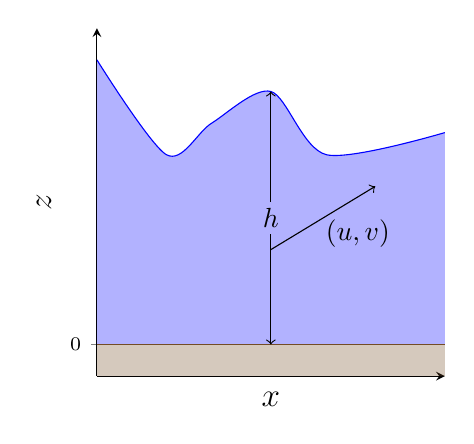
\begin{tikzpicture} 
	\begin{axis}[ 
	width = 0.7\textwidth,
	label style={font=\large},
	axis lines=left, xtick=\empty,
	ytick={0},
	clip mode=individual,
	xmin=0, 
	xmax=1, 
	width = 6cm,
	height = 6cm,
	ymin = -0.1, 
	ymax = 1,
	xlabel=$x$, 
	ylabel=$z$ ]
	%\addplot [blue] coordinates {(0,0.8)  (0.66,0.8)};
	\path[name path=axis] (axis cs:0,-0.1) -- (axis cs:1,-0.1);
	%\node[left] at (0,0.08) {$b$};
	\addplot [name path=b,brown!60!black, smooth] coordinates { (0,0.0)  (1,0.0)};
	
	\addplot [
	thick,
	color=brown!60!black,
	fill=brown!60!black, 
	fill opacity=0.3
	] fill between[of=b and axis];

	
	%\node[left] at (0,0.9) {$h$};
    \addplot [name path=h,blue, smooth] coordinates { (0,0.9) (0.2,0.6) (0.33,0.7) (0.5,0.8) (0.66,0.6) (1,0.67)};
    
   	\addplot [
   	thick,
   	color=blue,
   	fill=blue, 
   	fill opacity=0.3
   	] fill between[of=h and b];


	\addplot [<-,black] coordinates {(0.5,0.0) (0.5,0.35)};
	\node[] at (0.5,0.4) {$h$};
	\addplot [->,black] coordinates {(0.5,0.45) (0.5,0.8)};
	
	
	
	\addplot [->] coordinates {(0.5,0.3) (0.8,0.5)};
	\node[] at (0.75,0.35) {$(u,v)$};
	


	%\node[above right] at (0.6,0.4) {$\vec{u}$};
	%\addplot [->] coordinates {(0.5,0.5) (0.7,0.3)};
	
	\end{axis} 
	\end{tikzpicture} 
\end{document}